\chapter{Introduction}
\label{ch:intro}

In recent years, the world has seen an explosion in the amount of data. Initially, this data growth was triggered by the popularity of the Internet, but in the last few years, the growth of social networks such as Facebook, and micro-blogging services such as Twitter, have been responsible for producing ever-growing volumes of data. Over the same period of time, the declining cost of hardware has made it economically possible to set up sizable clusters of cheap computers to store and process this data. However, programming a cluster of shared-nothing computers is not an easy problem. Parallel programming has always been a hard problem, mostly owing to the lack of high-level abstractions to simplify the task.

Google, being at the forefront of this data-tsunami building a web-scale search engine, built the MapReduce \cite{mapreduce} programming model to enable their programmers to be productive on shared-nothing clusters. The MapReduce platform motivated the creation of the Hadoop \cite{hadoop:website}, an open source implementation of the MapReduce model. This development kick-started the new age of Big Data systems.

Initially, programmers used the MapReduce system to implement tools to quickly comb through very large amounts of data stored on clusters of commodity machines. Over time, it was clear that writing these tools in imperative languages, for analysis, was not the best use of programmers' time. To further improve programmer productivity, higher-level declarative languages were implemented (Sawzall~\cite{sawzall} and Tenzing~\cite{tenzing}, at Google, and Hive~\cite{hive}, at Facebook). The runtime layer used to process queries by these systems was still the MapReduce platform. While MapReduce was a simple model for programmers writing simple tools, we believed that it was the wrong layer for query language compilers to target, as their runtime layer. Sticking to the MapReduce abstraction forced queries to be evaluated as a sequence of MapReduce jobs with intermediate data materialized in a distributed filesystem, thus using a whole lot of unneeded resources. Several decades of database research has shown that pipelined architectures for executing queries consume fewer system resources, making better use of available hardware. One other problem with the MapReduce model was the reliance on unary operators for implementing Map and Reduce functions. This limitation of the model forces the need to express binary operations (such as joins) in an unnatural convoluted fashion. For example, Hive implements join over the MapReduce platform by expressing the operation as a grouping of the tagged union of the two relations being joined.
Another type of inefficiency introduced by the MapReduce platform has to do with the limited types of query processing algorithms that can be implemented within the framework, owing to the strict map-followed-by-sort-followed-by-reduce contract. For example, aggregation in MapReduce is implemented using a sort-based strategy because sorting is built into the system. A traditional parallel relational database system might have chosen a hash-based strategy to perform aggregation. This choice would require that the platform provide data redistribution primitives that offer more control. More details of these inefficiencies are described in Chapter~\ref{ch:hyracks}. Based on these observations, we designed and implemented Hyracks, a high-performance parallel dataflow runtime layer.

Hyracks was being built in the context of AsterixDB~\cite{ASTERIX}, a full-fledged, semi-structured, parallel big data management system that featured a fully functional declarative query language called AQL. As we started to build the query compilation layer for AQL, we realized that there was an opportunity to design the compilation framework in such a way that it could be re-purposed to build other declarative languages to be evaluated on the Hyracks platform. We called this layer Algebricks. Every query compiler built for parallel data-processing at the time (\cite{hive}, \cite{conf/sigmod/OlstonRSKT08}) was being built from scratch with its own parser, an intermediate representation based on an algebra, an optimizer to optimize queries, and finally a code generator to produce the runtime code. We designed Algebricks to provide an algebraic intermediate representation that was general enough to capture the semantics of the known languages, and also to be extensible to capture semantics of new, yet-to-come query languages of the future. Algebricks provides a rule-based optimizer and a library of generally applicable rewrite rules that can be used to quickly put together a compiler for a new declarative language. Algebricks also provides a code generator that compiles optimized queries to Hyracks jobs. Details of the Algebricks library can be found in Chapter~\ref{ch:algebricks}.

Figure~\ref{fig:asterixdb_stack} shows the various layers of the software stack that rests on the Hyracks platform. Algebricks, shown to the left of the figure, supports the AsterixDB compiler. In addition, we modified the Hive compiler to use Algebricks and run Hive queries as Hyracks jobs. Apache VXQuery~\cite{DBLP:conf/bigdataconf/CarmanWBCT15} is an open-source XQuery processor that has since been built to use Algebricks as its compilation framework to run queries over large amounts of XML data, on top of the Hyracks platform.

\begin{figure}[htb]
\centering
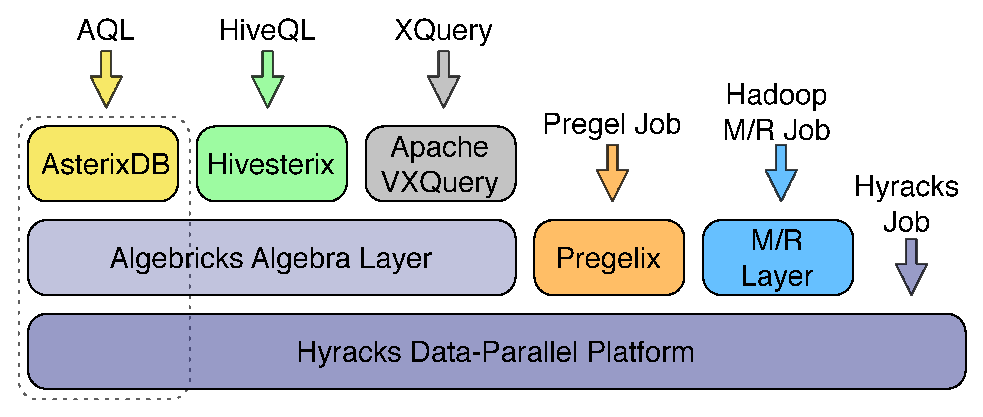
\includegraphics[width=6in]{images/asterixdb_stack}
%\vspace*{\betweenfigureandcaption}
\caption{Asterix software stack\label{fig:asterixdb_stack}}
%\vspace{-0.1in}
\end{figure}

Hyracks has also been successfully used to implement a clone of Pregel~\cite{Pregel}, called Pregelix~\cite{pregelix}. Pregelix implements a parallel framework to perform graph data processing at scale. Underneath, it uses Hyracks to implement the Pregel model using dataflow primitives. In terms of performance, it beats the foremost process-parallel open-source Pregel implementation called Giraph~\cite{giraph}. More details about the implementation of Pregelix are out of scope of this thesis, but can be found in \cite{pregelix}.

We proceed next to explore the related work in this area in Chapter~\ref{ch:foundations}. In Chapter~\ref{ch:hyracks} we describe the design and implementation of the Hyracks layer followed by that of Algebricks in Chapter~\ref{ch:algebricks}. Chapter~\ref{ch:asterixdb} describes how AsterixDB was built using Hyracks and Algebricks. Finally, we conclude in Chapter~\ref{ch:conclusions-and-future-work}.
